\begin{figure}[htbp]
\centering
\captionsetup{justification=raggedright,labelsep=none,singlelinecheck=false,labelformat=boldlabel}
\caption[Bibliographic networks of the review corpus]{\footnotesize \textbf{: Bibliographic networks of the review corpus.} Panel (a) is the co-citation network of the 25 most co-cited references, which identifies the knowledge base the corpus draws on. Panel (b) is the keyword co-occurrence network of the 25 most frequent terms. Both use the Fruchterman-Reingold layout with Salton normalization; node size is weighted degree and edge width is tie strength.}
\begin{subfigure}{\linewidth}\centering
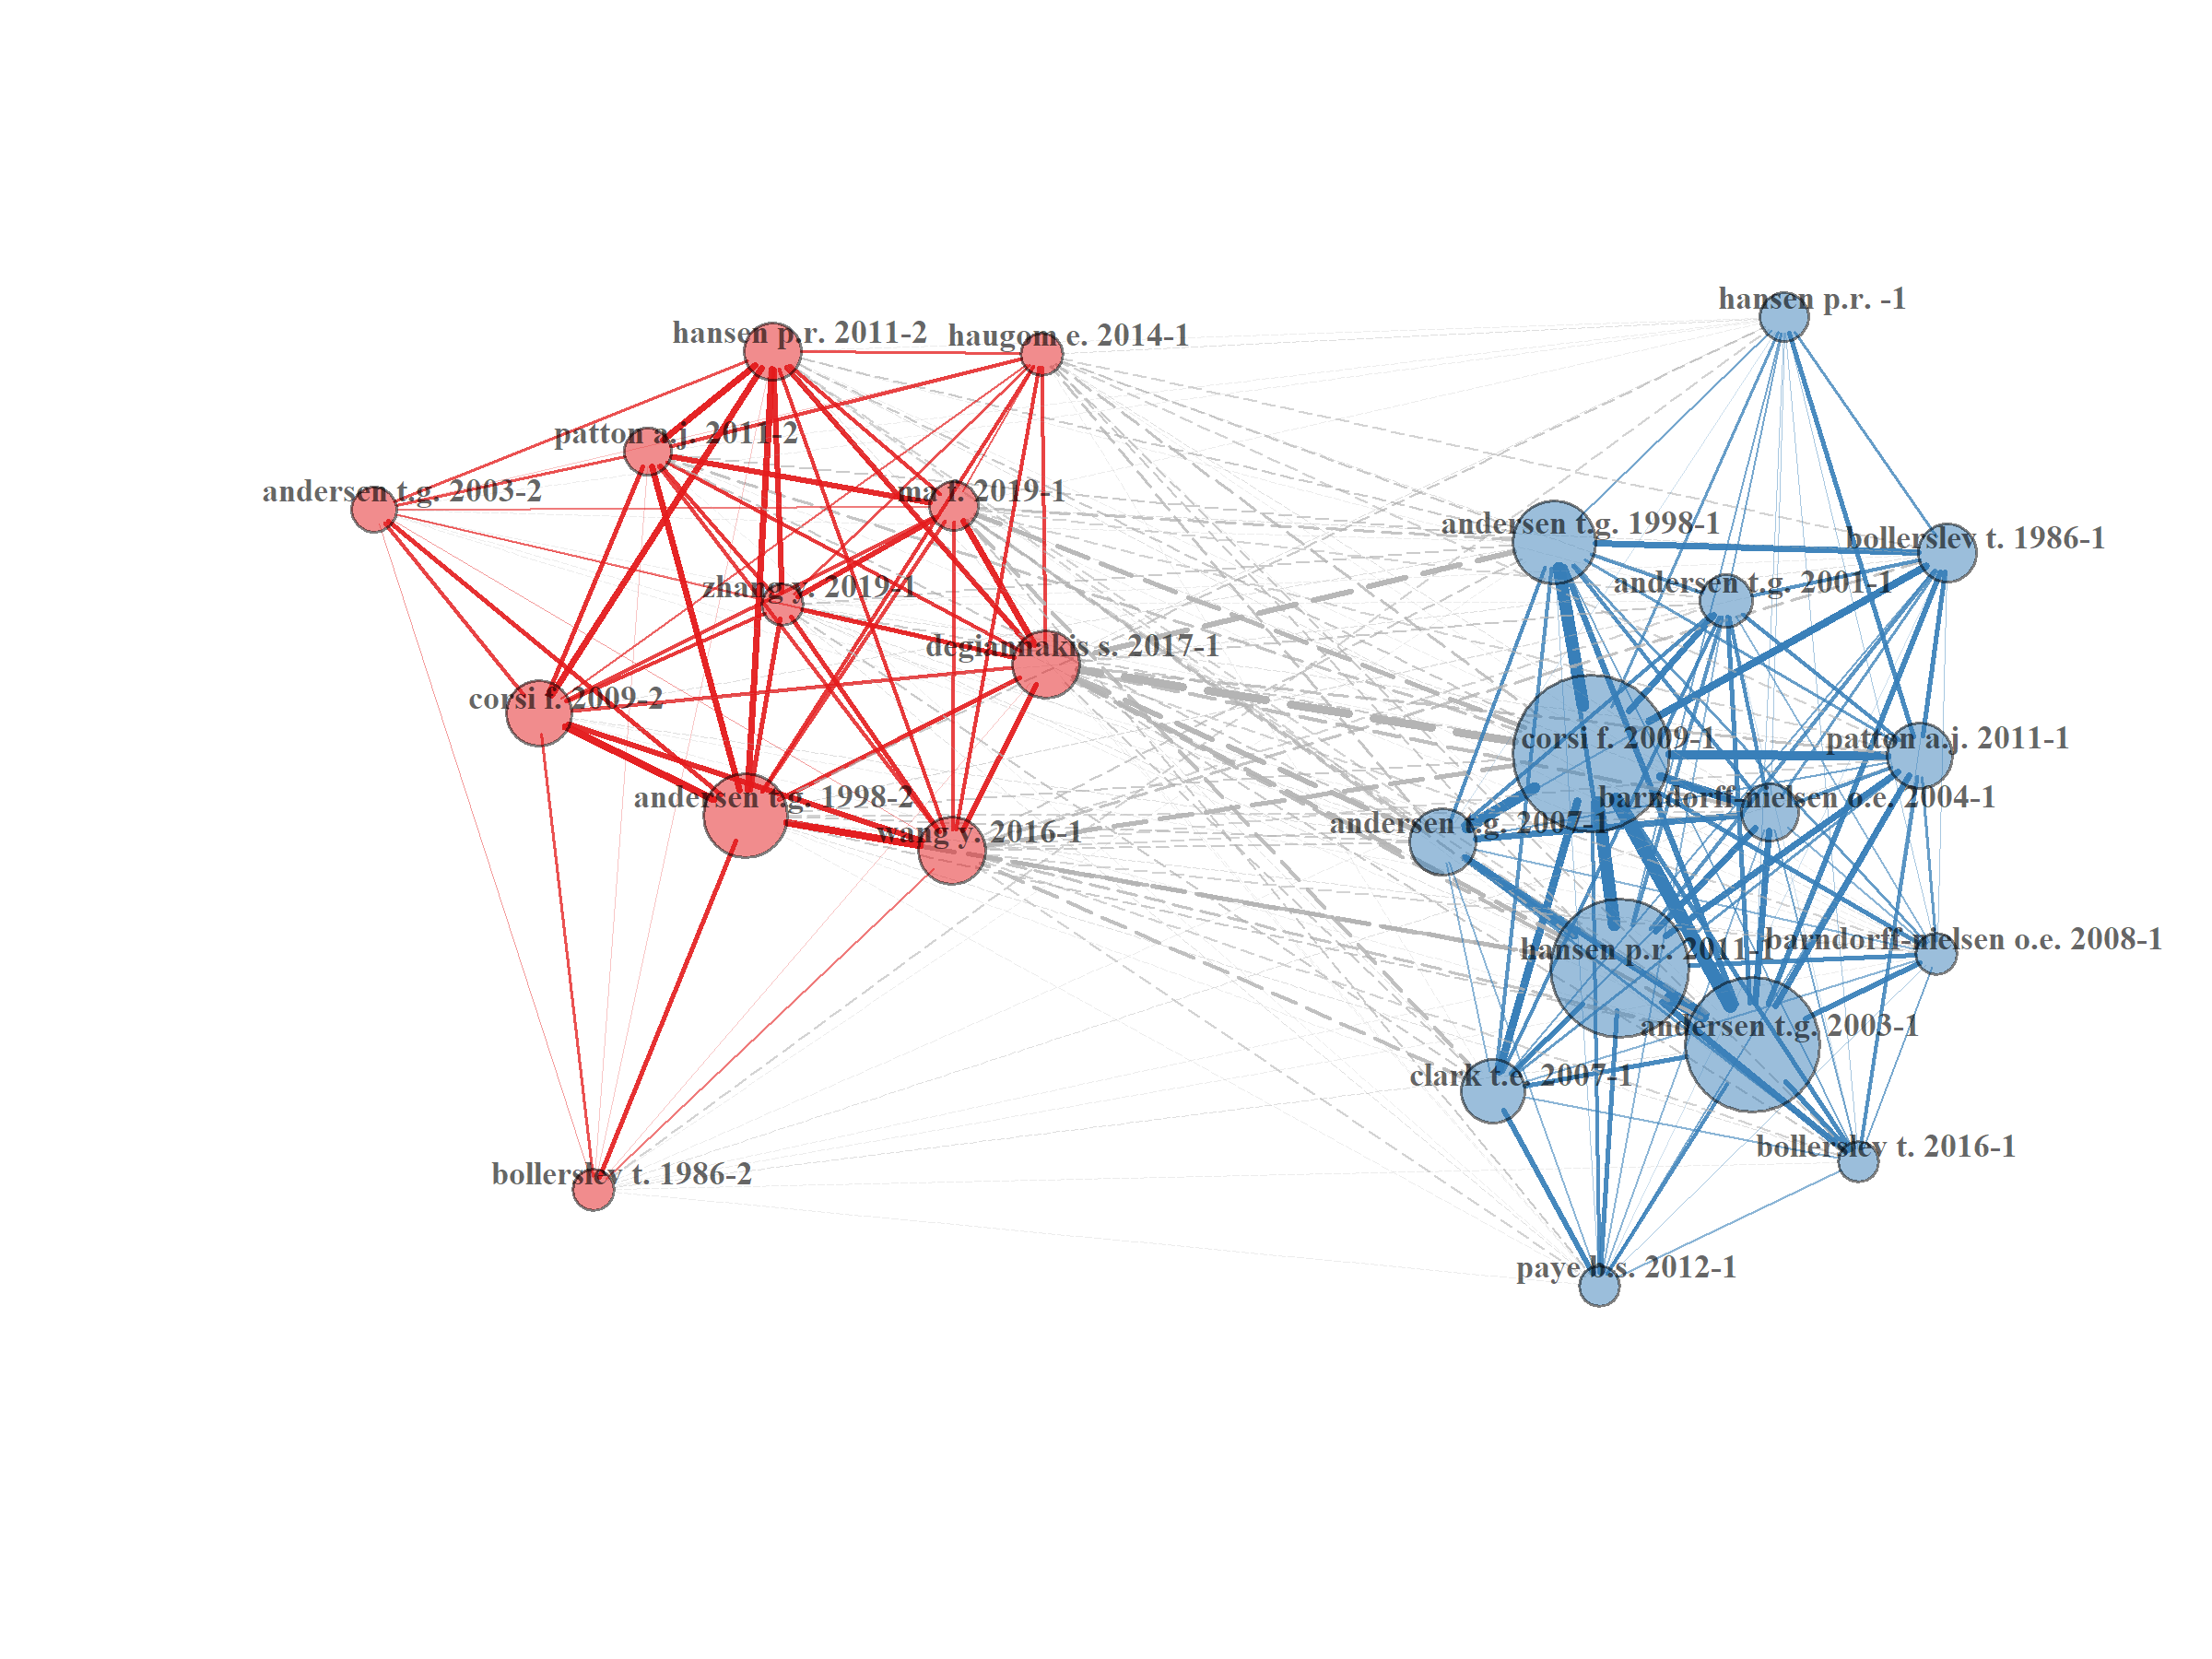
\includegraphics[width=0.86\linewidth]{figures/lit_cocitation.png}
\caption{Co-citation network}
\end{subfigure}
\begin{subfigure}{\linewidth}\centering
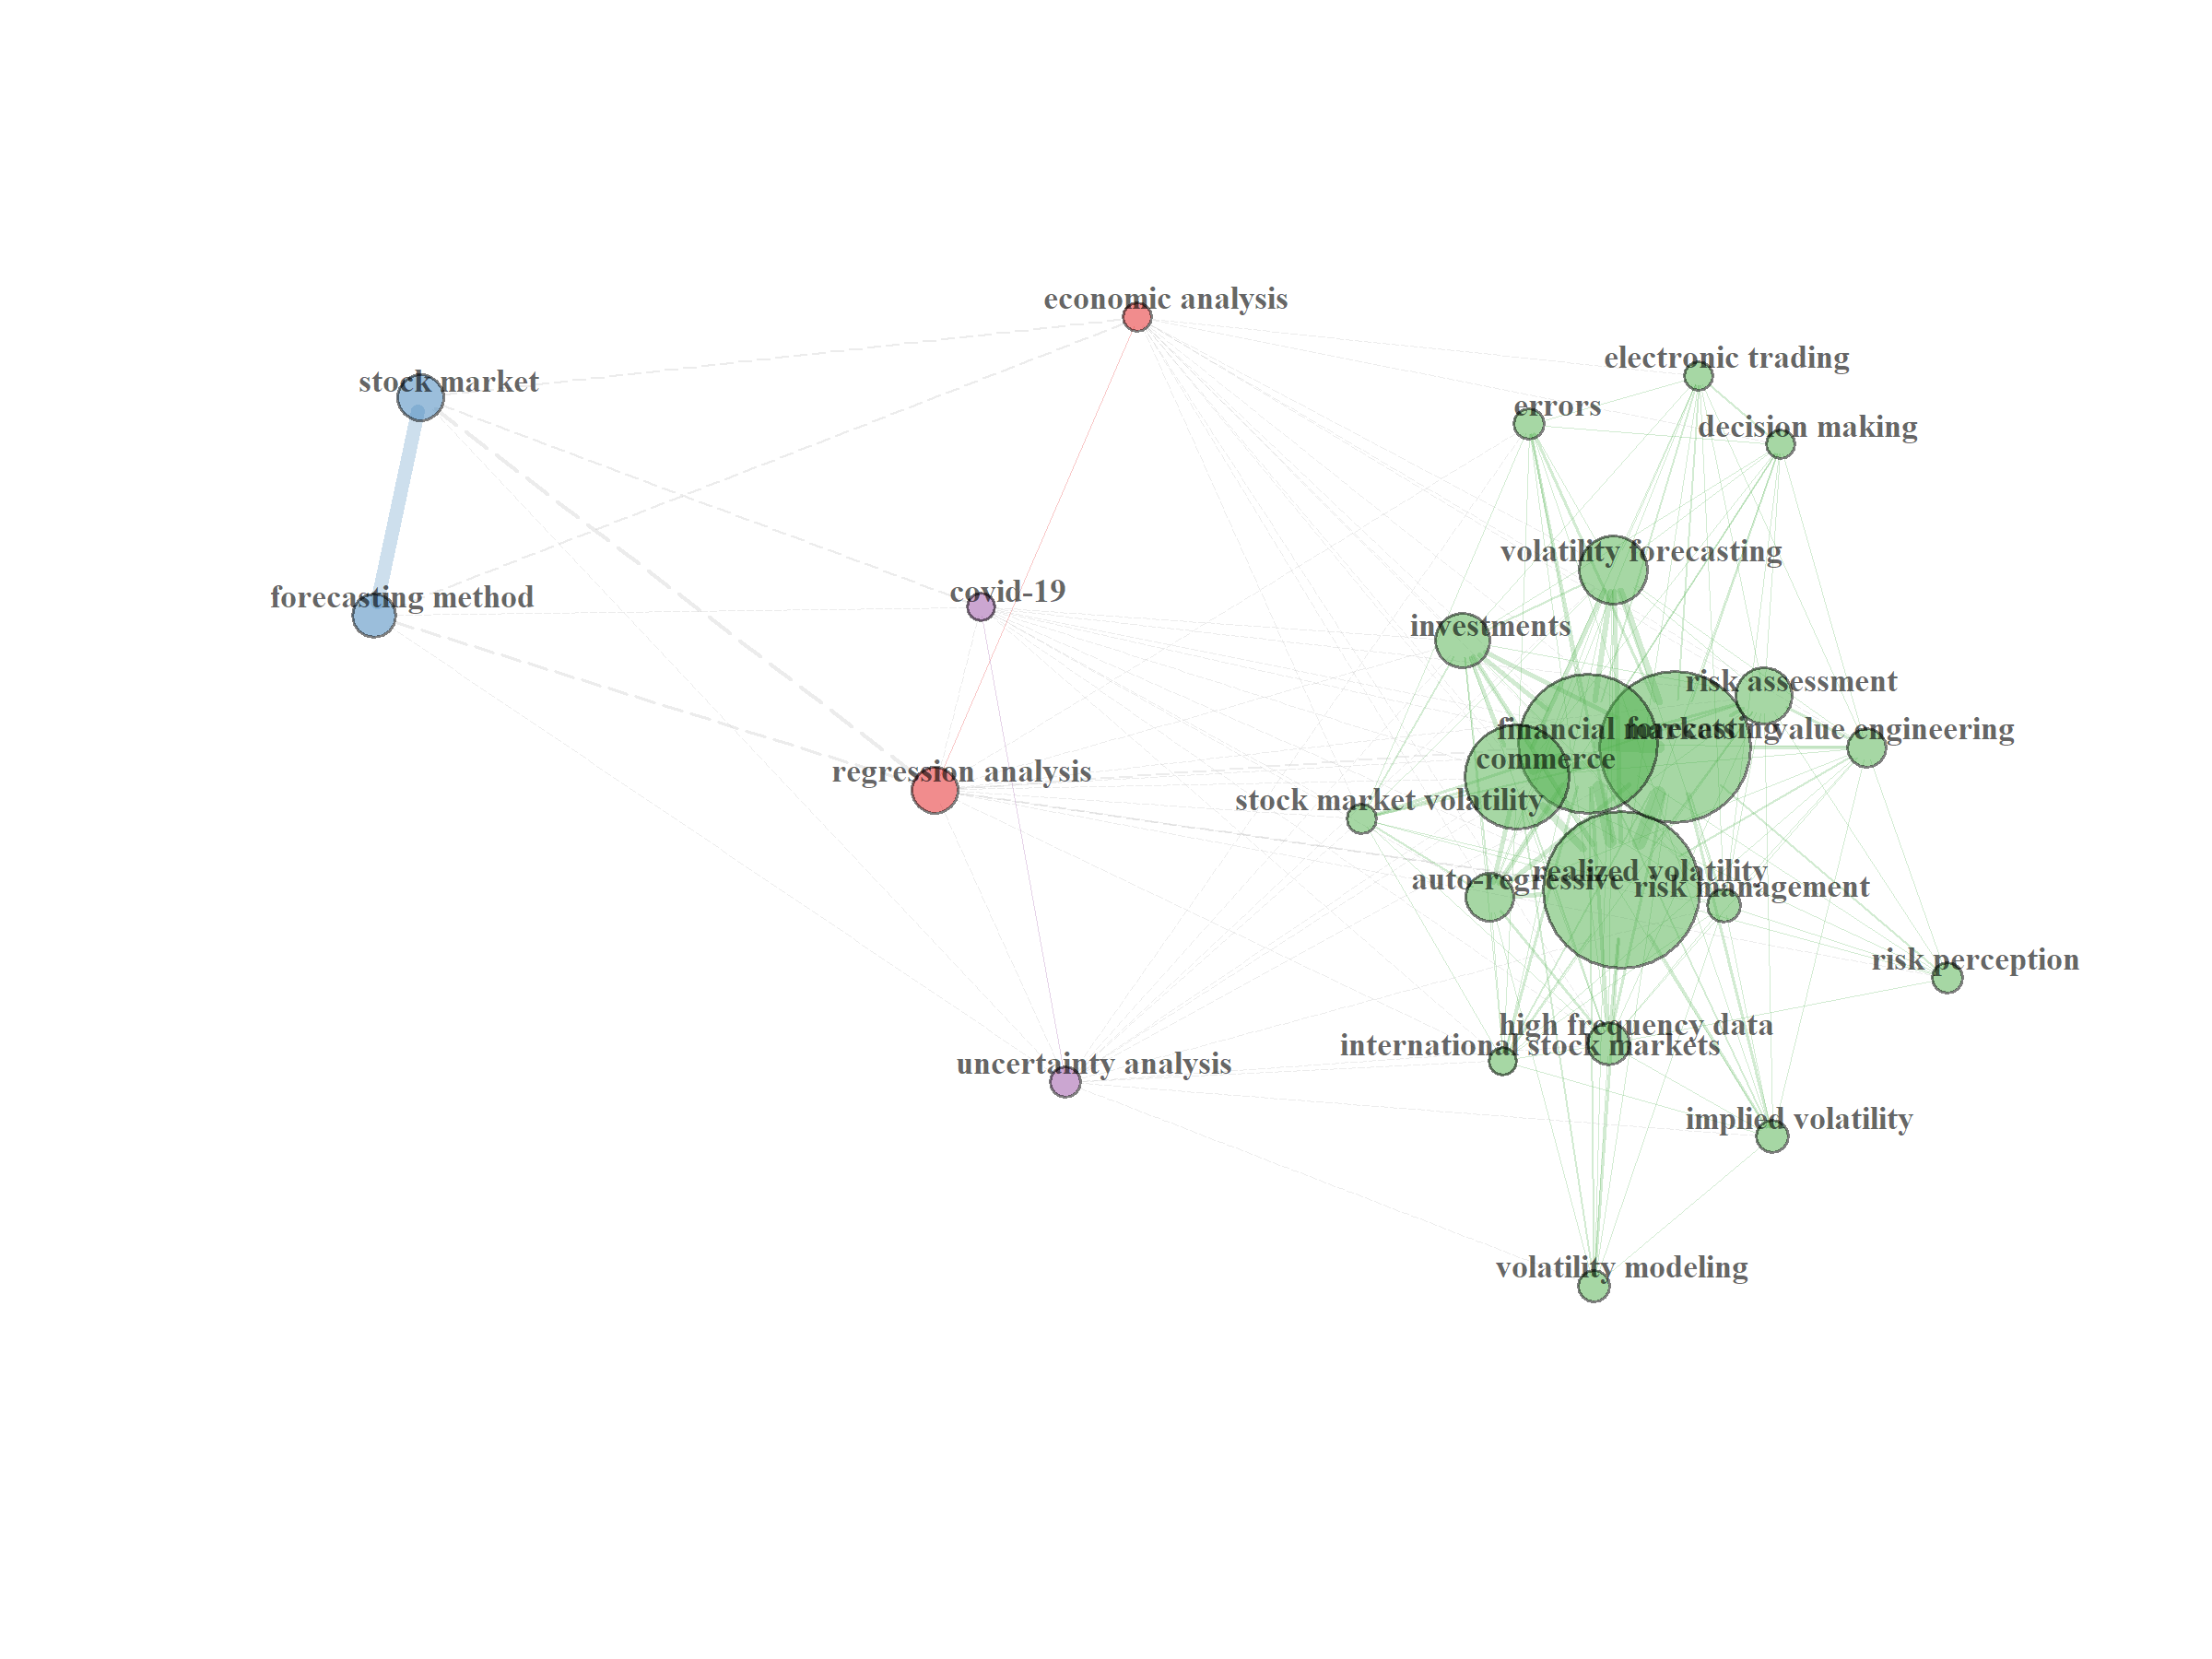
\includegraphics[width=0.86\linewidth]{figures/lit_keywords.png}
\caption{Keyword co-occurrence network}
\end{subfigure}
\label{fig:litnetworks}
\end{figure}
